% Final presentation -- work in progress, presented for critique (30 min + discussion).
% Slot moved to Wednesday, November 4, 2026, 08:20.
% No animations and no screenshots of papers: equations are typeset in LaTeX.
\documentclass[aspectratio=169,11pt,xcolor=table]{beamer}

\usepackage[utf8]{inputenc}
\IfFileExists{spanish.ldf}{\usepackage[spanish,es-nodecimaldot,es-noshorthands,es-lcroman]{babel}}{}
\IfFileExists{lmodern.sty}{\usepackage[T1]{fontenc}\usepackage{lmodern}}{}
\usepackage{amsmath,amssymb}
\usepackage{bbm}
\usepackage{booktabs}
\usepackage{array}
\usepackage{tabularx}
\newcolumntype{L}[1]{>{\raggedright\arraybackslash}p{#1}}
\newcolumntype{Y}{>{\raggedright\arraybackslash}X}
\usepackage{graphicx}
\usepackage{tikz}
\usetikzlibrary{positioning,arrows.meta,decorations.pathreplacing}
\usepackage{newunicodechar}
% Lean code is full of Unicode that typewriter fonts do not have. Each line
% maps one symbol to math mode, so Lean can be pasted into a verbatim block
% as it is (inside a [fragile] frame). Add a line for any symbol you need.
\newunicodechar{∀}{\ensuremath{\forall}}  \newunicodechar{∃}{\ensuremath{\exists}}
\newunicodechar{→}{\ensuremath{\to}}      \newunicodechar{↔}{\ensuremath{\leftrightarrow}}
\newunicodechar{∧}{\ensuremath{\land}}    \newunicodechar{∨}{\ensuremath{\lor}}
\newunicodechar{¬}{\ensuremath{\lnot}}    \newunicodechar{×}{\ensuremath{\times}}
\newunicodechar{∈}{\ensuremath{\in}}      \newunicodechar{∉}{\ensuremath{\notin}}
\newunicodechar{≤}{\ensuremath{\le}}      \newunicodechar{≥}{\ensuremath{\ge}}
\newunicodechar{≠}{\ensuremath{\ne}}      \newunicodechar{↦}{\ensuremath{\mapsto}}
\newunicodechar{ℝ}{\ensuremath{\mathbb{R}}} \newunicodechar{ℕ}{\ensuremath{\mathbb{N}}}
\newunicodechar{⟨}{\ensuremath{\langle}}  \newunicodechar{⟩}{\ensuremath{\rangle}}
\newunicodechar{λ}{\ensuremath{\lambda}}  \newunicodechar{α}{\ensuremath{\alpha}}
\newunicodechar{β}{\ensuremath{\beta}}    \newunicodechar{ε}{\ensuremath{\varepsilon}}
\newunicodechar{ρ}{\ensuremath{\rho}}     \newunicodechar{κ}{\ensuremath{\kappa}}
\newunicodechar{τ}{\ensuremath{\tau}}     \newunicodechar{η}{\ensuremath{\eta}}
\newunicodechar{μ}{\ensuremath{\mu}}      \newunicodechar{∑}{\ensuremath{\sum}}
\newunicodechar{₀}{\ensuremath{_0}}       \newunicodechar{₁}{\ensuremath{_1}}
\newunicodechar{⁻}{\ensuremath{^{-}}}     \newunicodechar{¹}{\ensuremath{^{1}}}
\newunicodechar{Δ}{\ensuremath{\Delta}}   \newunicodechar{ω}{\ensuremath{\omega}}
\newunicodechar{θ}{\ensuremath{\theta}}   \newunicodechar{∏}{\ensuremath{\prod}}
\newunicodechar{·}{\ensuremath{\cdot}}

% ---------------- Estilo (el de la tesis) ----------------
\definecolor{upblue}{HTML}{1E3A8A}
\definecolor{upaccent}{HTML}{2E6FD8}
\definecolor{upgray}{HTML}{5B6170}
\definecolor{upred}{HTML}{C0392B}
\definecolor{uplight}{HTML}{EEF2FA}

\usetheme{default}
\setbeamertemplate{navigation symbols}{}
\setbeamercolor{frametitle}{fg=upblue}
\setbeamerfont{frametitle}{series=\bfseries,size=\Large}
\setbeamercolor{structure}{fg=upblue}
\setbeamercolor{normal text}{fg=black!85}
\setbeamercolor{alerted text}{fg=upred}
\setbeamertemplate{itemize items}{\color{upaccent}$\blacktriangleright$}
\setbeamertemplate{itemize subitem}{\color{upgray}--}
\newcommand{\itemgap}{0.9em}
\makeatletter
\let\OLDitemize\itemize
\renewcommand\itemize{\OLDitemize\ifnum\@itemdepth=1\setlength{\itemsep}{\itemgap}\else\setlength{\itemsep}{0.4em}\setlength{\topsep}{0.5em}\fi}
\makeatother
\setbeamercolor{block title}{bg=upblue,fg=white}
\setbeamercolor{block body}{bg=uplight}
\setbeamertemplate{blocks}[rounded][shadow=false]
\setbeamertemplate{frametitle}{%
  \vspace{0.35cm}\insertframetitle\par
  \vspace{-0.1cm}{\color{upaccent}\rule{2.2cm}{1.5pt}}%
}
\setbeamertemplate{footline}{%
  \hbox{\begin{beamercolorbox}[wd=\paperwidth,ht=3ex,dp=1.2ex]{}%
    \hfill{\color{upgray}\tiny\insertframenumber/\inserttotalframenumber}\hspace{0.4cm}%
  \end{beamercolorbox}}%
}
\newcommand{\hl}[1]{\textcolor{upaccent}{\textbf{#1}}}
\newcommand{\E}{\mathbb{E}}
\newcommand{\1}{\mathbbm{1}}
\newcommand{\pending}[1]{\textcolor{upred}{\textbf{[Pendiente: #1]}}}
\IfFileExists{../code/output/numbers.tex}{\newcommand{\tauShareMin}{18}
\newcommand{\tauShareMax}{22}
\newcommand{\tauMin}{0.05}
\newcommand{\tauMax}{0.09}
\newcommand{\DeltaDataMin}{0.25}
\newcommand{\DeltaDataMax}{0.46}
\newcommand{\habitDecayMax}{0.009}
\newcommand{\objMzero}{1{,}451}
\newcommand{\objMone}{1{,}430}
\newcommand{\objBest}{1{,}276}
\newcommand{\bestModel}{M2}
\newcommand{\betaStatic}{2.22}
\newcommand{\betaBest}{1.37}
\newcommand{\lamBest}{0.37}
\newcommand{\rhoBest}{0.95}
\newcommand{\peakBest}{43}
\newcommand{\nMoments}{222}
}{}

\title{La brecha de participación a los 70 años sobrestima el efecto del voto obligatorio}
\subtitle{Ciclo de vida, hábito y una calibración con datos de la ONPE}
\author{Manuel Alfredo Arriola Montenegro}
\date{4 de noviembre de 2026}

\begin{document}

% ===== Portada =====
{
\setbeamertemplate{footline}{}
\begin{frame}
  \begin{center}
    
\includegraphics[height=1.3cm]{logo.png}\\[0.5cm]
    {\color{upblue}\Large\bfseries La brecha de participación a los 70 años\\ sobrestima el efecto del voto obligatorio}\\[0.2cm]
    {\color{upgray}\large \insertsubtitle}\\[0.5cm]
    {\small\textbf{Manuel Alfredo Arriola Montenegro}}\\[0.2cm]
    {\small Presentación final (trabajo en progreso) \;\textbar\; Track B: modelo de tesis}\\[0.15cm]
    {\footnotesize\color{upgray} Inteligencia Artificial y Modelamiento Económico \;\textbar\; Lima, 4 de noviembre de 2026}\\[0.25cm]
    {\small\color{upaccent}\href{https://github.com/Arriola123456/ai-project}{\texttt{github.com/Arriola123456/ai-project}}}
  \end{center}
\end{frame}
}

% ===== 1. Pregunta y resultado =====
\begin{frame}{1. La pregunta y el resultado en una frase}
  \begin{block}{Pregunta}
    En el Perú el voto es facultativo desde los 70 años. ¿Qué mide la brecha de participación entre
    los grupos de 60--69 y 70+ que reporta la ONPE?
  \end{block}
  \vspace{0.2cm}
  \begin{block}{Resultado}
    La brecha $\Delta$ es una \textbf{cota superior} del efecto causal $\tau^{70}$ de la obligación,
    \textbf{siempre que} el índice total de beneficio, \alert{incluido el hábito}, no crezca entre
    los 60 y los 70 años.
  \end{block}
  \vspace{0.2cm}
  \begin{itemize}
    \item En los datos: la brecha entre grupos es de 25 a 46 pp; el salto en el umbral $\theta_{70}$, de 5 a 12 pp.
    \item Que el beneficio decrezca con la edad \textbf{no basta}: si el hábito todavía se acumula, $\Delta<\tau^{70}$ es posible.
  \end{itemize}
\end{frame}

% ===== 2. Modelo =====
\begin{frame}{2. El modelo: el cálculo del voto con edad y hábito}
  \small Elecciones cada $d=5$ años. El ciudadano $i$, de edad $a$, elige $v\in\{0,1\}$ en la elección $t$:
  \begin{block}{Problema del ciudadano}
    \[
      \max_{v\in\{0,1\}}\; v\bigl[b(a)+\lambda h_{it}-c_{it}\bigr]+(1-v)\bigl[-O_a S_t\bigr],
      \qquad O_a=\1[a<70],\quad S_t=s_0+qF_t
    \]
  \end{block}
  \begin{columns}[T]
    \begin{column}{0.48\textwidth}
      \begin{itemize}\setlength{\itemsep}{0.4em}
        \item \hl{Beneficio por edad}: $b(a)=A a^{\alpha}-\kappa a^{\beta}$, con $0<\alpha<1\le\beta$.
        \item \hl{Costo}: $c_{it}=\mu_t+\eta_i+\varepsilon_{it}$ (persistente + transitorio).
      \end{itemize}
    \end{column}
    \begin{column}{0.48\textwidth}
      \begin{itemize}\setlength{\itemsep}{0.4em}
        \item \hl{Hábito}: $h_{i,t+1}=\rho(a_{it})\,h_{it}+v_{it}$, el shock es el voto anterior.
        \item \hl{Miopía}: no internaliza el efecto del voto sobre su hábito.
      \end{itemize}
    \end{column}
  \end{columns}
  \begin{block}{Condición de corte (análogo de la CPO)}
    \centering $v_{it}=1\iff \varepsilon_{it}<b(a)+\lambda h_{it}+O_aS_t-\mu_t-\eta_i$
  \end{block}
\end{frame}

\begin{frame}{2. Dos objetos distintos: $\tau^{70}$ y $\Delta$}
  \begin{columns}[T]
    \begin{column}{0.48\textwidth}
      \begin{block}{Efecto causal en el umbral}
        \[ \tau^{70}=\E\bigl[G(\bar c+S)-G(\bar c)\bigr],\]
        \[ \bar c=b(70)+\lambda h_{70}-\mu-\eta \]
        \footnotesize Los mismos ciudadanos a los 70, \textbf{con su hábito acumulado}, con y sin obligación.
      \end{block}
    \end{column}
    \begin{column}{0.48\textwidth}
      \begin{block}{Lo que reporta la ONPE}
        \[ \Delta=\E_{a\in[60,70)}\bigl[P(a)\bigr]-\E_{a\ge 70}\bigl[P(a)\bigr] \]
        \footnotesize Promedios sobre la distribución de electores por edad dentro de cada grupo.
      \end{block}
    \end{column}
  \end{columns}
  \vspace{0.3cm}
  \begin{itemize}
    \item Datos de la tesis: perfiles $\theta_a=P(a)-P(69)$ por \textbf{edad exacta}, con efectos fijos de mesa, en 10 elecciones presidenciales.
    \item $\theta_{70}$ es el salto más un año de envejecimiento; $\Delta$ es lo que mide la brecha por grupos.
  \end{itemize}
\end{frame}

% ===== 3. Proposiciones =====
\begin{frame}{3. Proposición 1: el ciclo de vida}
  \begin{block}{Proposición 1 \quad (Supuesto 1: $A,\kappa>0$, $0<\alpha<1\le\beta$)}
    $b$ es estrictamente cóncava y tiene un máximo único en
    \[ a^*=\Bigl(\tfrac{A\alpha}{\kappa\beta}\Bigr)^{1/(\beta-\alpha)} . \]
    Con $\beta=1$, $b'(a)\to-\kappa$ (caída lineal); con $\beta>1$, $b'(a)\to-\infty$ (caída que se acelera).
  \end{block}
  \begin{itemize}
    \item Prueba: $b'(a)=a^{\alpha-1}\bigl[A\alpha-\kappa\beta a^{\beta-\alpha}\bigr]$ cambia de signo una sola vez.
    \item ¿Conviene $\beta>1$? Es lo que decide la calibración: sin hábito, los datos empujan $\beta$ a su cota.
  \end{itemize}
\end{frame}

\begin{frame}{3. Lema 1 y Proposición 2: el salto}
  \begin{block}{Lema 1: acoplamiento \quad ($\lambda\ge0$, $S\ge0$, $\rho\ge0$)}
    Con los mismos shocks, si $0\le\lambda\le\lambda'$ y los umbrales $\theta_j\le\theta'_j$ en cada elección,
    las trayectorias de hábito quedan ordenadas, $0\le h_j\le h'_j$, y quien vota en el primer entorno vota en el segundo.
  \end{block}
  \begin{block}{Proposición 2: el salto no contiene hábito}
    A los 70 el hábito se acumuló bajo obligación. Si $g$ es unimodal con moda $m$ y $\bar c\ge m$ en todo el soporte,
    $\tau^{70}$ es \textbf{no creciente en $\lambda$}: el hábito atenúa el salto.
  \end{block}
  {\small Prueba: el Lema 1 sube $\bar c$; $G$ es cóncava sobre la moda, así que $G(x+S)-G(x)$ baja.}
\end{frame}

\begin{frame}{3. Proposición 3: la brecha es una cota superior}
  \begin{block}{Proposición 3 \quad (Supuestos 1--4, $\lambda\ge0$, $S\ge0$)}
    $P_1(a)$: participación si hoy fuera obligatoria; $P^f(a)$, $a\ge70$: con todas las elecciones pasadas obligadas.
    Bajo \textbf{(H)}: $P_1$ no creciente en $[60,70]$ y $P^f$ no creciente en $[70,\infty)$,
    \begin{gather*}
      \Delta=\tau^{70}+\mathcal{E}+\mathcal{D}\;\ge\;\tau^{70},\\
      \mathcal{E}=[\bar P_{60\text{--}69}-P_1(70)]+[P^f(70)-\bar P^f_{70+}]\ge0,\qquad
      \mathcal{D}=\bar P^f_{70+}-\bar P_{70+}\ge0 .
    \end{gather*}
  \end{block}
  \begin{itemize}\setlength{\itemsep}{0.4em}
    \item $\mathcal{E}$ es envejecimiento dentro de cada banda; $\mathcal{D}$, el decaimiento del hábito tras la exención (Lema 1).
    \item (H) es sobre el índice \textbf{total} $b(a)+\lambda h$. Con $a^*\le 60$ y nada más hay contraejemplos (punto 7).
  \end{itemize}
\end{frame}

\begin{frame}{3. Proposiciones 4 y 5: la huella del hábito}
  {\small Entorno estacionario ($\mu_t=\mu$, $S_t=S$): la participación a la edad $x$ en una elección pasada es la misma $P(x)$.}
  \begin{block}{Proposición 4: escalones cada $d$ años ($\rho$ constante, identidad exacta)}
    $H(a)=\E[h]=\sum_{k\ge0}\rho^{k}P(a-(k+1)d)$ y, si $a+1-18$ no es múltiplo de $d$,
    \[ H(a+1)-H(a)=\sum_{k\ge0}\rho^{k}\bigl[P(a+1-(k+1)d)-P(a-(k+1)d)\bigr]. \]
    \footnotesize Entre 74 y 75 el término $k=0$ es $P(70)-P(69)$: \textbf{el salto vuelve como un escalón}.
  \end{block}
  \begin{block}{Proposición 5: persistencia creciente, $\rho'(a)\ge0$, $\Pi_k(a)=\prod_{j=1}^{k}\rho(a-jd)$}
    \[ H(a+1)-H(a)=\sum_{k\ge0}\Pi_k(a+1)\bigl[P(a+1-(k+1)d)-P(a-(k+1)d)\bigr]+\alert{R(a)},\quad R(a)\ge0 . \]
    \footnotesize El salto entra en el escalón de $70+(k+1)d$ con peso $\ge\rho(70)^k$: se propaga \textbf{más} que con $\rho$ constante.
  \end{block}
\end{frame}

% ===== 4. La prueba =====
\begin{frame}{4. La prueba: qué está hecho y qué sigue abierto}
  \begin{columns}[T]
    \begin{column}{0.32\textwidth}
      {\color{upblue}\bfseries Hecho}
      \begin{itemize}\setlength{\itemsep}{0.4em}\small
        \item Pruebas completas de P1--P5 y del Lema 1, \textbf{también en Lean}, sin \texttt{sorry}.
        \item P2, P3: por acoplamiento (mismos shocks, trayectorias ordenadas).
        \item P4, P5: forma cerrada del AR(1) por linealidad de la esperanza.
      \end{itemize}
    \end{column}
    \begin{column}{0.32\textwidth}
      {\color{upred}\bfseries Lo difícil}
      \begin{itemize}\setlength{\itemsep}{0.4em}\small
        \item La hipótesis correcta de P3: con hábito, ``$b$ decreciente'' no alcanza.
        \item Los supuestos que las pruebas usaban sin decirlo: $\lambda\ge0$, $S\ge0$ y la estacionariedad de P4--P5.
        \item El resto $R(a)$ de P5, que apareció al escribirla en Lean.
      \end{itemize}
    \end{column}
    \begin{column}{0.32\textwidth}
      {\color{upgray}\bfseries Abierto}
      \begin{itemize}\setlength{\itemsep}{0.4em}\small
        \item Una condición sobre primitivas que implique (H).
        \item P4--P5 con $\mu_t$ y $S_t$ que cambian entre elecciones.
        \item Versión con votante que mira hacia adelante.
      \end{itemize}
    \end{column}
  \end{columns}
\end{frame}

% ===== 5. Simulaciones y calibración =====
\begin{frame}{5. Calibración al estilo DSGE}
  \begin{itemize}\setlength{\itemsep}{0.5em}
    \item \textbf{Externos}: $d=5$; la multa $F_t$ en \% de la UIT, ponderada por electores (JNE): 4\% antes de la Ley 28859 y 1.8--1.9\% después.
    \item \textbf{Comunes a las elecciones}: $a^*,\alpha,\kappa,\beta,\lambda,\rho_0,\rho_1,\omega,s_0,q$. \textbf{Por elección}: el nivel $\mu_t$.
    \item \textbf{Momentos}: $\theta_a$ para las edades 45--80, ponderados por $1/\text{ee}^2$, y los niveles de las bandas 60--69 y 70+, en 6 elecciones (2001 2V y 1V 2006--2026).
    \item \textbf{Modelos anidados}: M0 estático con $\beta=1$ $\subset$ M1 $\beta$ libre $\subset$ M2 hábito $\subset$ M3 $\rho(a)$ creciente.
    \item Robustez: todas las edades 20--80 y todas las bandas.
  \end{itemize}
\end{frame}

\begin{frame}{5. Resultados de la calibración}
  \centering\small
  \IfFileExists{../code/output/calib_models.tex}{\resizebox{\textwidth}{!}{\begin{tabular}{lrrrrrrrrr}
\toprule
Modelo & Objetivo & $a^*$ & $\alpha$ & $\beta$ & $\lambda$ & $\rho_0$ & $\rho_1$ & $s_0$ & $q$ \\
\midrule
M0: estático{,} $\beta=1$ & 1{,}451 & 53.6 & 0.98 & -- & -- & -- & -- & 0.25 & 0.00 \\
M1: estático{,} $\beta$ libre & 1{,}430 & 53.3 & 0.98 & 2.22 & -- & -- & -- & 0.24 & 0.00 \\
M2: hábito{,} $\rho$ constante & 1{,}276 & 43.0 & 0.64 & 1.37 & 0.37 & 0.95 & -- & 0.29 & 0.00 \\
M3: hábito{,} $\rho(a)$ creciente & 1{,}276 & 43.0 & 0.56 & 1.44 & 0.37 & 0.95 & 0.00 & 0.29 & 0.00 \\
\bottomrule
\end{tabular}}}{\pending{tabla de modelos}}
  \vspace{0.3cm}
  \raggedright
  \begin{itemize}\setlength{\itemsep}{0.35em}
    \item ¿Conviene $\beta>1$? Poco: de \objMzero{} a \objMone{} ($\beta=\betaStatic$). El hábito aporta más (\objBest{}).
    \item $\rho_0=\rhoBest$, en su cota: el hábito que piden los datos es casi permanente. \textbf{$\rho'(a)>0$ no mejora nada} ($\rho_1\to0$): la persistencia ya está saturada.
    \item $q\approx0$: la multa no explica el salto. En 2006, con multa de 4\% UIT, $\theta_{70}=-0.063$; en 2021, con 1.9\%, $-0.118$.
  \end{itemize}
\end{frame}

\begin{frame}[c]{5. Ajuste a los perfiles por edad}
  \centering
  \IfFileExists{../code/figures/fit_profiles.pdf}{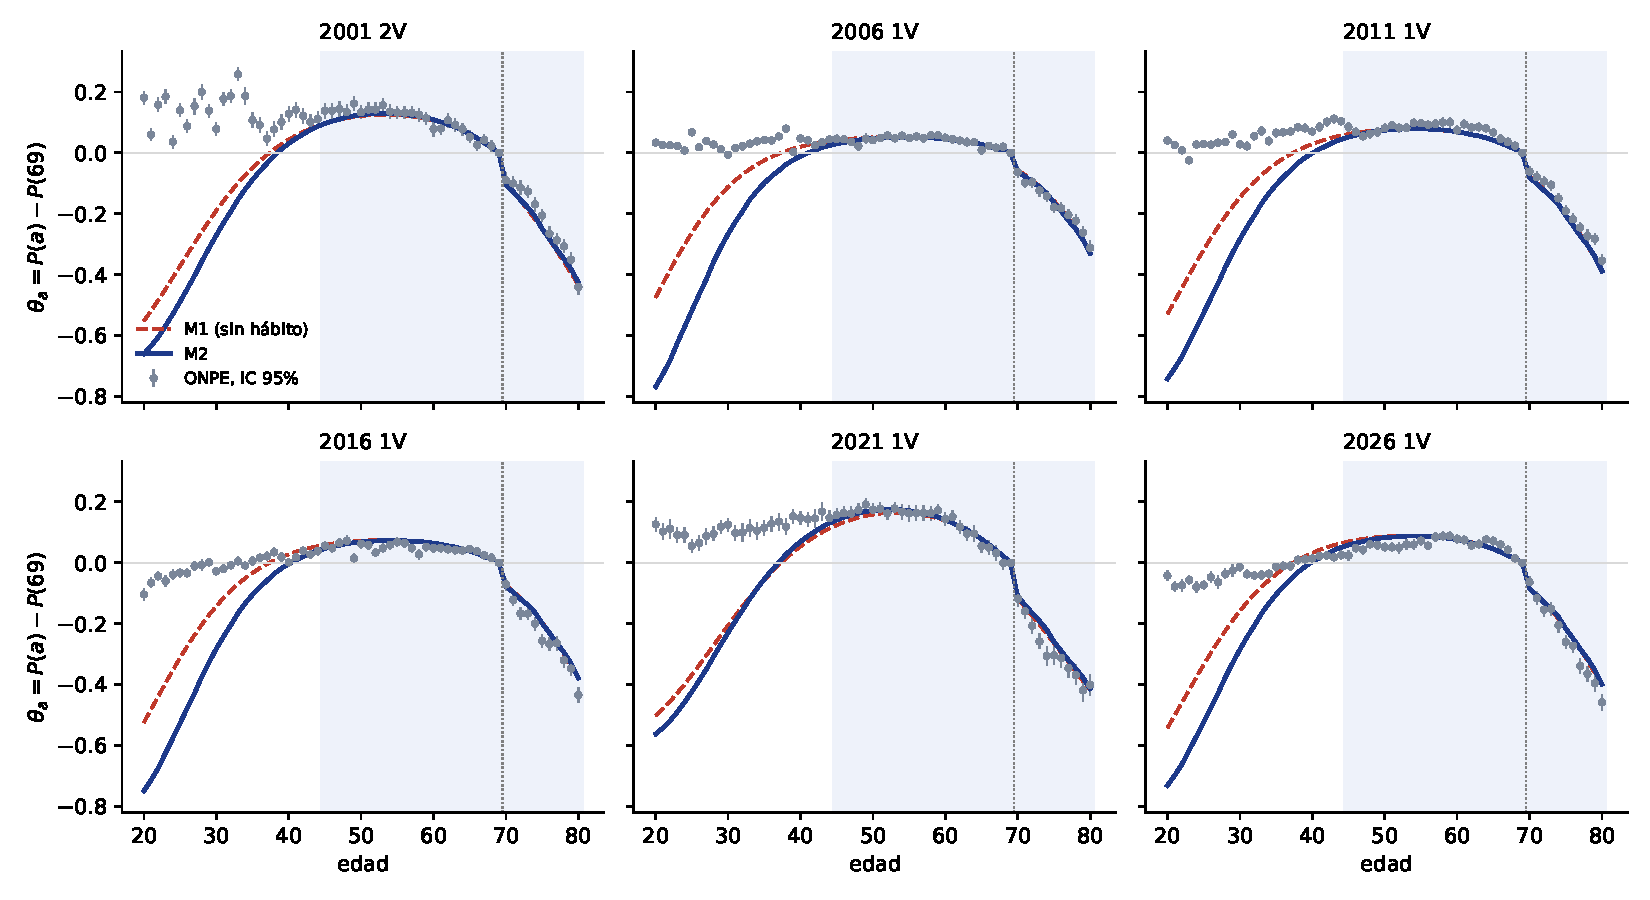
\includegraphics[width=0.92\textwidth,height=0.78\textheight,keepaspectratio]{../code/figures/fit_profiles.pdf}}{\pending{figura de ajuste}}
\end{frame}

\begin{frame}{5. ¿Cuánto de la brecha es causal?}
  \centering\small
  \IfFileExists{../code/output/gap_table.tex}{\resizebox{\textwidth}{!}{\begin{tabular}{lrrrrrrr}
\toprule
 & \multicolumn{2}{c}{$\theta_{70}$} & \multicolumn{2}{c}{$\Delta$} & \multicolumn{3}{c}{Descomposición de $\Delta$ (modelo)} \\
\cmidrule(lr){2-3}\cmidrule(lr){4-5}\cmidrule(lr){6-8}
Elección & datos & modelo & datos & modelo & $\tau^{70}$ & envejec. & hábito \\
\midrule
2001 2V & -0.090 & -0.104 & 0.323 & 0.384 & 0.083 & 0.293 & 0.008 \\
2006 1V & -0.063 & -0.062 & 0.250 & 0.267 & 0.052 & 0.208 & 0.007 \\
2011 1V & -0.062 & -0.081 & 0.313 & 0.342 & 0.067 & 0.266 & 0.009 \\
2016 1V & -0.071 & -0.078 & 0.365 & 0.356 & 0.064 & 0.282 & 0.009 \\
2021 1V & -0.118 & -0.112 & 0.459 & 0.416 & 0.089 & 0.321 & 0.007 \\
2026 1V & -0.064 & -0.086 & 0.393 & 0.374 & 0.071 & 0.295 & 0.009 \\
\bottomrule
\end{tabular}}}{\pending{descomposición}}
  \vspace{0.3cm}
  \begin{block}{Lectura}
    El efecto causal es $\tau^{70}\in[\tauMin,\tauMax]$: \textbf{solo el \tauShareMin--\tauShareMax\% de la brecha}.
    El resto es envejecimiento dentro de la banda abierta 70+. El decaimiento del hábito aporta poco (a lo más \habitDecayMax).
  \end{block}
\end{frame}

\begin{frame}{5. Qué verifican las simulaciones y qué no pueden mostrar}
  \begin{columns}[T]
    \begin{column}{0.48\textwidth}
      {\color{upblue}\bfseries \texttt{code/verify.py} verifica}
      \begin{itemize}\setlength{\itemsep}{0.4em}\small
        \item P1 y (a)--(d) con SymPy.
        \item P2--P5 con el modelo: las identidades de P4 y P5 al error de máquina.
        \item Contraejemplos: (iv) con promedios, turno 5 de claude.ai, P3 sin (H) y P5 sin $R(a)$.
        \item La calibración se reproduce desde \texttt{code/data/} y respeta el anidamiento.
      \end{itemize}
    \end{column}
    \begin{column}{0.48\textwidth}
      {\color{upred}\bfseries Lo que no puede mostrar}
      \begin{itemize}\setlength{\itemsep}{0.4em}\small
        \item Una simulación sobre una grilla de parámetros no es una prueba.
        \item La calibración no identifica cohortes: el corte transversal mezcla edad y cohorte.
        \item El padrón con fallecidos baja la participación medida de 70+.
      \end{itemize}
    \end{column}
  \end{columns}
\end{frame}

% ===== 6. Lean =====
\begin{frame}[fragile]{6. Lean: la Proposición 3, del paper a Lean}
  \small\textbf{En el paper.} Bajo (H), $\Delta=\tau^{70}+\mathcal{E}+\mathcal{D}$ con $\mathcal{E}\ge0$ y $\mathcal{D}\ge0$, así que $\Delta\ge\tau^{70}$.

  \textbf{En Lean} (\texttt{lean/PaperInterface.lean}). $P$, $P_1$ y $P^f$ se definen desde las primitivas: la regla de corte,
  la recursión del hábito con las edades $a-(n-j)d$ y una población finita con pesos.
{\footnotesize
\begin{verbatim}
  (∀ a a', 60 ≤ a → a ≤ a' → a' ≤ 70 → P1 a' ≤ P1 a) →   -- (H), parte 1
  (∀ a a', 70 ≤ a → a ≤ a' → Pf a' ≤ Pf a) →              -- (H), parte 2
  Δ = τ + E + D ∧ 0 ≤ E ∧ 0 ≤ D ∧ τ ≤ Δ
\end{verbatim}}
  \textbf{El paso clave} (\texttt{lean/ProofInterface.lean}): la historia obligada domina a la observada.
{\footnotesize
\begin{verbatim}
  obtain ⟨-, hle, -⟩ := lemma1_coupling (fun j => ρ (age a j))
    (fun j => base ω (age a j) + O (age a j) * S)   -- observada
    (fun j => base ω (age a j) + S)                 -- obligada
    (ε ω a) lam lam (hobs ω a) (hcomp ω a) ...
\end{verbatim}}
  \textbf{Qué verifica Lean.} El enunciado del paper, con sus mismas hipótesis: (H), $\lambda\ge0$, $S\ge0$, $\rho\ge0$, $G$ creciente.
  Lo único que agrega es representar la esperanza como un promedio sobre una población finita.
\end{frame}

\begin{frame}{6. Lean: el estado de cada resultado}
  \centering\small
  \begin{tabular}{llll}
    \toprule
    Resultado & Declaración en Lean & Estado & Qué se agrega \\
    \midrule
    Lema 1 & \texttt{lemma1\_coupling} & probado & -- \\
    Proposición 1 & \texttt{prop1\_lifecycle} & probado & -- \\
    Proposición 2 & \texttt{prop2\_jump} & probado & población finita \\
    Proposición 3 & \texttt{prop3\_bound} & probado & población finita \\
    Proposición 4 & \texttt{prop4\_steps} & probado & población finita \\
    Proposición 5 & \texttt{prop5\_rising\_persistence} & probado & población finita \\
    \bottomrule
  \end{tabular}

  \vspace{0.4cm}\raggedright
  \begin{itemize}\setlength{\itemsep}{0.4em}
    \item \IfFileExists{../lean/docs/CHECK_FAST_OUTPUT.txt}{\texttt{lake build} y \texttt{check --fast} sin errores; ningún \texttt{sorry}.}{\pending{resultado de \texttt{check --fast}}}
    \item La estacionariedad de P4--P5 no es una hipótesis agregada: está en el paper como supuesto.
    \item Corrida de AppliedModelingLib hecha por Claude Code, no por GPT-5.6 Sol (declarado en \texttt{prompts.md}).
  \end{itemize}
\end{frame}

% ===== 7. Dónde no le creí a la IA =====
\begin{frame}{7. Dónde no le creí a la IA (1): la hipótesis de P3}
  \begin{block}{Lo que afirmó el modelo (Claude Code, al plantear P3)}
    ``Si $a^*\le 60$ y el hábito es estacionario bajo obligación, entonces $\Delta\ge\tau^{70}$.''
  \end{block}
  \begin{itemize}\setlength{\itemsep}{0.5em}
    \item \textbf{Veredicto: falso tal como estaba.} Con elecciones cada 5 años, el hábito no es estacionario a los 60 ($\rho^8$ no es despreciable).
    \item El índice $b(a)+\lambda\E[h_a]$ puede crecer entre 60 y 70 aunque $b$ decrezca: hay 7 de 150 sorteos con $a^*\le 60$ y $\Delta<\tau^{70}$.
    \item \textbf{Corrección}: la hipótesis (H) se pone sobre la participación, no sobre $b$.
    \item Antes ya habían caído (iv) con promedios por grupo y el turno 5 de la sesión de claude.ai.
  \end{itemize}
\end{frame}

\begin{frame}{7. Dónde no le creí a la IA (2): el resto de P5}
  \begin{block}{Lo que afirmó el modelo (primer borrador de P5)}
    ``Con $\rho$ creciente, la identidad de P4 vale reemplazando $\rho^k$ por el producto de las persistencias.''
  \end{block}
  \small A mano, con $\Pi_k(a)=\prod_{j=1}^{k}\rho(a-jd)$ y $H(a)=\sum_k\Pi_k(a)P(a-(k+1)d)$:
  {\footnotesize
  \begin{align*}
    H(a+1)-H(a)&=\textstyle\sum_k\bigl[\Pi_k(a+1)P(a+1-(k+1)d)-\Pi_k(a)P(a-(k+1)d)\bigr]\\
    &=\textstyle\sum_k\Pi_k(a+1)\bigl[P(a+1-(k+1)d)-P(a-(k+1)d)\bigr]+R(a),\\
    R(a)&=\textstyle\sum_k\bigl[\Pi_k(a+1)-\Pi_k(a)\bigr]P(a-(k+1)d)\;\ge\;0\quad\text{si }\rho'\ge0 .
  \end{align*}}
  \begin{itemize}\setlength{\itemsep}{0.2em}
    \item \textbf{Veredicto: falso.} Los coeficientes dependen de la edad de hoy, $a$ o $a+1$. Sin $R(a)$, el error llega a $\PfiveNaiveErr$ (\texttt{verify.py}).
    \item Salió al escribir el enunciado para Lean, que ahora prueba la versión con $R(a)$.
  \end{itemize}
  \pending{foto de la derivación a mano (\texttt{hand/})}
\end{frame}

% ===== 8. Preguntas =====
\begin{frame}{8. Dónde quiero su crítica}
  \begin{enumerate}\setlength{\itemsep}{0.9em}
    \item ¿Es razonable el ciudadano \textbf{miope}? Con mirada hacia adelante, votar hoy tiene valor de opción por el hábito.
    \item Las edades menores de 45 varían entre elecciones de forma que ningún ciclo de vida captura. ¿Es legítimo calibrar solo la ventana 45--80, o eso es elegir los momentos a conveniencia?
    \item ¿Qué contraste empírico separa el hábito de un $\beta$ alto: los escalones de la Proposición 4, o algo más?
  \end{enumerate}
\end{frame}

{
\setbeamertemplate{footline}{}
\begin{frame}[c]
  \begin{center}
    {\color{upblue}\Huge\bfseries Gracias}\\[0.3cm]
    {\large Comentarios y crítica}\\[0.8cm]
    Manuel Alfredo Arriola Montenegro\\[0.1cm]
    {\small\color{upaccent}\texttt{github.com/Arriola123456/ai-project}}\\[0.3cm]
    
\includegraphics[height=1cm]{logo.png}
  \end{center}
\end{frame}
}

\end{document}
